%
% This document contains the chapter about non-linear devices.
%
% Copyright (C) 2003, 2004, 2005 Stefan Jahn <stefan@lkcc.org>
%
% Permission is granted to copy, distribute and/or modify this document
% under the terms of the GNU Free Documentation License, Version 1.1
% or any later version published by the Free Software Foundation.
%

\chapter{Non-linear devices}
%\addcontentsline{toc}{chapter}{Non-linear devices}
\label{sec:NLdevices}

\section{PN-Junction Diode}
%\addcontentsline{toc}{section}{PN-Junction Diode}

The following table contains the model parameters for the pn-junction
diode model.

\addvspace{12pt}

\begin{tabular}{rllll}
Name & Symbol & Description & Unit & Default\\
\hline
Is & $I_{S}$ & saturation current & $\ampere$ & $10^{-14}$\\
N & $N$ & emission coefficient & & $1.0$\\
Isr & $I_{SR}$ & recombination current parameter & $\ampere$ & $0.0$\\
Nr & $N_{R}$ & emission coefficient for Isr & & $2.0$\\
Rs & $R_{S}$ & ohmic resistance & $\ohm$ & $0.0$\\
Cj0 & $C_{j0}$ & zero-bias junction capacitance & $\farad$ & $0.0$\\
M & $M$ & grading coefficient & & $0.5$\\
Vj & $V_{j}$ & junction potential & $\volt$ & $0.7$\\
Fc & $F_{c}$ & forward-bias depletion capacitance coefficient & & $0.5$\\
Cp & $C_{p}$ & linear capacitance & $\farad$ & $0.0$\\
Tt & $\tau$ & transit time & $\second$ & $0.0$\\
Kf & $K_F$ & flicker noise coefficient & & $0.0$\\
Af & $A_F$ & flicker noise exponent & & $1.0$\\
Ffe & $F_{FE}$ & flicker noise frequency exponent & & $1.0$\\
Temp & $T$ & device temperature & $\degree \mathrm{C}$ & $26.85$
\end{tabular}

\addvspace{12pt}

\subsection{Large signal model}
%\addcontentsline{toc}{subsection}{Large signal model}

\begin{figure}[ht]
\begin{center}
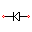
\includegraphics[width=0.3\linewidth]{diode}
\end{center}
\caption{pn-junction diode symbol and large signal model}
\label{fig:diode}
\end{figure}
\FloatBarrier

The current equation of the diode and its derivative writes as
follows:
\begin{align}
I_{d} &= I_{S}\cdot \left(e^{\frac{V_{d}}{N\cdot V_{T}}} - 1\right) + I_{SR}\cdot \left(e^{\frac{V_{d}}{N_R\cdot V_{T}}} - 1\right)\\
g_{d} &= \dfrac{\partial I_{d}}{\partial V_{d}} = \dfrac{I_{S}}{N\cdot V_{T}}\cdot e^{\frac{V_{d}}{N\cdot V_{T}}} + \dfrac{I_{SR}}{N_R\cdot V_{T}}\cdot e^{\frac{V_{d}}{N_R\cdot V_{T}}}
\end{align}

\begin{figure}[ht]
\begin{center}
\includegraphics[width=0.17\linewidth]{dcdiode}
\end{center}
\caption{accompanied DC model of intrinsic diode}
\label{fig:dcdiode}
\end{figure}
\FloatBarrier

The complete MNA matrix entries are:
\begin{equation}
\begin{bmatrix}
g_{d} & -g_{d}\\
-g_{d} & g_{d}\\
\end{bmatrix}
\cdot
\begin{bmatrix}
V_{C}\\
V_{A}\\
\end{bmatrix}
=
\begin{bmatrix}
+I_{d} - g_{d}\cdot V_{d}\\
-I_{d} + g_{d}\cdot V_{d}\\
\end{bmatrix}
\end{equation}

\subsection{Small signal model}
%\addcontentsline{toc}{subsection}{Small signal model}

\begin{figure}[ht]
\begin{center}
\includegraphics[width=0.17\linewidth]{spdiode}
\end{center}
\caption{small signal model of intrinsic diode}
\label{fig:spdiode}
\end{figure}
\FloatBarrier

The voltage dependent capacitance consists of a diffusion capacitance,
a junction capacitance and an additional linear capacitance which is
usually modeled by the following equations.

\begin{equation}
C_{d} = C_p + \tau \cdot g_{d} +
\begin{cases}
\begin{array}{ll}
C_{j0}\cdot \left(1 - \dfrac{V_{d}}{V_{j}}\right)^{-M} & \textrm{ for } V_{d} \le F_c\cdot V_j\\
\dfrac{C_{j0}}{\left(1 - F_c\right)^M}\cdot \left(1 + \dfrac{M\cdot \left(V_{d} - F_c\cdot V_j\right)}{V_{j}\cdot\left(1 - F_c\right)}\right) & \textrm{ for } V_{d} > F_c\cdot V_j
\end{array}
\end{cases}
\end{equation}

The S-parameters of the passive circuit shown in
fig. \ref{fig:spdiode} can be written as
\begin{align}
S_{11} = S_{22} &= \dfrac{1}{1 + 2\cdot y}\\
S_{12} = S_{21} &= 1 - S_{11} = \dfrac{2\cdot y}{1 + 2\cdot y}
\end{align}

with
\begin{equation}
y = Z_{0}\cdot \left(g_{d} + j\omega C_{d}\right)
\end{equation}

\subsection{Noise model}
%\addcontentsline{toc}{subsection}{Noise model}

The thermal noise generated by the series resistor is characterized by
the following spectral density.
\begin{equation}
\dfrac{\overline{i_{R_S}^2}}{\Delta f} = \dfrac{4 k_B T}{R_S}
\end{equation}

\begin{figure}[ht]
\begin{center}
\includegraphics[width=0.28\linewidth]{noisediode}
\end{center}
\caption{noise model of intrinsic diode}
\label{fig:noisediode}
\end{figure}
\FloatBarrier

The shot noise and flicker noise generated by the DC current flow
through the diode is characterized by the following spectral density.
\begin{equation}
\dfrac{\overline{i_{d}^2}}{\Delta f} = 2e I_d + K_F \dfrac{I_d^{A_F}}{f^{F_{FE}}}
\end{equation}

Thus the noise current correlation matrix can be formed.  This matrix
can be easily converted to the noise wave correlation matrix
representation using the formulas given in section
\ref{sec:noiseTrans} on page \pageref{sec:noiseTrans}.
\begin{equation}
\underline{C}_Y = \Delta f
\begin{bmatrix}
+\overline{i_{d}^2} & -\overline{i_{d}^2}\\
-\overline{i_{d}^2} & +\overline{i_{d}^2}\\
\end{bmatrix}
\end{equation}

\section{Junction FET}
%\addcontentsline{toc}{section}{Junction FET}

The following table contains the model parameters for the JFET model.

\addvspace{12pt}

\begin{tabular}{rllll}
Name & Symbol & Description & Unit & Default\\
\hline
Vt0 & $V_{Th}$ & zero -bias threshold voltage & $\volt$ & $-2.0$\\
Beta & $\beta$ & transconductance parameter & $\ampere / \volt^{2}$ & $10^{-4}$\\
Lambda & $\lambda$ & channel-length modulation parameter & $1/\volt$ & $0.0$\\
Rd & $R_{D}$ & drain ohmic resistance & $\ohm$ & $0.0$\\
Rs & $R_{S}$ & source ohmic resistance & $\ohm$ & $0.0$\\
Is & $I_{S}$ & gate-junction saturation current & $\ampere$ & $10^{-14}$\\
N & $N$ & gate P-N emission coefficient & & $1.0$\\
Isr & $I_{SR}$ & gate-junction recombination current parameter & $\ampere$ & $0.0$\\
Nr & $N_{R}$ & Isr emission coefficient & & $2.0$\\
Cgs & $C_{gs}$ & zero-bias gate-source junction capacitance & $\farad$ & $0.0$\\
Cgd & $C_{gd}$ & zero-bias gate-drain junction capacitance & $\farad$ & $0.0$\\
Pb & $P_{b}$ & gate-junction potential & $\volt$ & $1.0$\\
Fc & $F_{c}$ & forward-bias junction capacitance coefficient & & $0.5$\\
M & $M$ & gate P-N grading coefficient & & $0.5$\\
Kf & $K_F$ & flicker noise coefficient & & $0.0$\\
Af & $A_F$ & flicker noise exponent & & $1.0$\\
Ffe & $F_{FE}$ & flicker noise frequency exponent & & $1.0$\\
Temp & $T$ & device temperature & $\degree \mathrm{C}$ & $26.85$
\end{tabular}

\addvspace{12pt}

\subsection{Large signal model}
%\addcontentsline{toc}{subsection}{Large signal model}

\begin{figure}[ht]
\begin{center}
\includegraphics[width=0.5\linewidth]{jfet}
\end{center}
\caption{junction FET symbol and large signal model}
\label{fig:jfet}
\end{figure}
\FloatBarrier

The current equation of the gate source diode and its derivative
writes as follows:
\begin{align}
I_{GS} &= I_{S}\cdot \left(e^{\frac{V_{GS}}{N\cdot V_{T}}} - 1\right) + I_{SR}\cdot \left(e^{\frac{V_{GS}}{N_{R}\cdot V_{T}}} - 1\right)\\
g_{gs} &= \dfrac{\partial I_{GS}}{\partial V_{GS}} = \dfrac{I_{S}}{N\cdot V_{T}}\cdot e^{\frac{V_{GS}}{N\cdot V_{T}}} + \dfrac{I_{SR}}{N_{R}\cdot V_{T}}\cdot e^{\frac{V_{GS}}{N_{R}\cdot V_{T}}}
\end{align}

The current equation of the gate drain diode and its derivative writes
as follows:
\begin{align}
I_{GD} &= I_{S}\cdot \left(e^{\frac{V_{GD}}{N\cdot V_{T}}} - 1\right) + I_{SR}\cdot \left(e^{\frac{V_{GD}}{N_{R}\cdot V_{T}}} - 1\right)\\
g_{gd} &= \dfrac{\partial I_{GD}}{\partial V_{GD}} = \dfrac{I_{S}}{N\cdot V_{T}}\cdot e^{\frac{V_{GD}}{N\cdot V_{T}}} + \dfrac{I_{SR}}{N_{R}\cdot V_{T}}\cdot e^{\frac{V_{GD}}{N_{R}\cdot V_{T}}}
\end{align}

Both equations contain the gate-junction saturation current $I_{S}$,
the gate P-N emission coefficient $N$ and the temperature voltage
$V_{T}$ with the Boltzmann's constant $k_{B}$ and the electron charge
$q$.  The operating temperature $T$ must be specified in Kelvin.
\begin{equation}
V_{T} = \dfrac{k_{B}\cdot T}{q}
\end{equation}

The controlled drain currents have been defined by Shichman and Hodges
\cite{Shichman} for different modes of operations.

\begin{equation}
g_{m} = \dfrac{\partial I_{d}}{\partial V_{GS}}
\;\;\;\; \text{ and } \;\;\;\;
g_{ds} = \dfrac{\partial I_{d}}{\partial V_{DS}}
\;\;\;\; \text{ with } \;\;\;\;
V_{GD} = V_{GS} - V_{DS}
\end{equation}

\begin{itemize}
\item normal mode: $V_{DS} > 0$
\begin{itemize}
\item normal mode, cutoff region: $V_{GS} - V_{Th} < 0$
\begin{align}
I_{d} &= 0\\
g_{m} &= 0\\
g_{ds} &= 0\\
%\end{align}
\intertext{
\item normal mode, saturation region: $0 < V_{GS} - V_{Th} < V_{DS}$
}
%\begin{align}
I_{d} &= \beta \cdot\left(1 + \lambda V_{DS}\right) \cdot\left(V_{GS} - V_{Th}\right)^{2}\\
g_{m} &= \beta \cdot\left(1 + \lambda V_{DS}\right) \cdot 2\left(V_{GS} - V_{Th}\right)\\
g_{ds} &= \beta \cdot \lambda\left(V_{GS} - V_{Th}\right)^{2}\\
%\end{align}
\intertext{
\item normal mode, linear region: $V_{DS} < V_{GS} - V_{Th}$
}
%\begin{align}
I_{d} &= \beta\cdot\left(1 + \lambda V_{DS}\right)\cdot\left(2 \left(V_{GS} - V_{Th}\right) - V_{DS}\right)\cdot V_{DS}\\
g_{m} &= \beta\cdot\left(1 + \lambda V_{DS}\right)\cdot 2\cdot V_{DS}\\
g_{ds} &= \beta\cdot\left(1 + \lambda V_{DS}\right)\cdot 2\left(V_{GS} - V_{Th} - V_{DS}\right) + \beta \cdot \lambda V_{DS}\cdot\left(2\left(V_{GS} - V_{Th}\right) - V_{DS}\right)
\end{align}
\end{itemize}
\item inverse mode: $V_{DS} < 0$
\begin{itemize}
\item inverse mode, cutoff region: $V_{GD} - V_{Th} < 0$
\begin{align}
I_{d} &= 0\\
g_{m} &= 0\\
g_{ds} &= 0\\
%\end{align}
\intertext{
\item inverse mode, saturation region: $0 < V_{GD} - V_{Th} < -V_{DS}$
}
%\begin{align}
I_{d} &= -\beta \cdot\left(1 - \lambda V_{DS}\right) \cdot\left(V_{GD} - V_{Th}\right)^{2}\\
g_{m} &= -\beta \cdot\left(1 - \lambda V_{DS}\right) \cdot 2\left(V_{GD} - V_{Th}\right)\\
g_{ds} &= \beta \cdot\lambda \left(V_{GD} - V_{Th}\right)^{2} + \beta\cdot\left(1 - \lambda V_{DS}\right) \cdot 2\left(V_{GD} - V_{Th}\right)\\
%\end{align}
\intertext{
\item inverse mode, linear region: $-V_{DS} < V_{GD} - V_{Th}$
}
%\begin{align}
I_{d} &= \beta\cdot\left(1 - \lambda V_{DS}\right)\cdot\left(2 \left(V_{GD} - V_{Th}\right) + V_{DS}\right)\cdot V_{DS}\\
g_{m} &= \beta\cdot\left(1 - \lambda V_{DS}\right)\cdot 2\cdot V_{DS}\\
g_{ds} &= \beta\cdot\left(1 - \lambda V_{DS}\right)\cdot 2\left(V_{GD} - V_{Th}\right) - \beta \cdot \lambda V_{DS}\cdot\left(2\left(V_{GD} - V_{Th}\right) + V_{DS}\right)
\end{align}
\end{itemize}
\end{itemize}

The MNA matrix entries for the voltage controlled drain current source
can be written as:

\addvspace{12pt}

\begin{center}
\begin{tabular}{p{1.5cm}|lll}
\raggedleft & \centering G & \centering S & controlling nodes\\
\hline
\raggedleft D & $+g_{m}$ & $-g_{m}$ &\\
\raggedleft S & $-g_{m}$ & $+g_{m}$ &\\
\raggedleft controlled nodes & & &
\end{tabular}
\end{center}

\addvspace{12pt}

With the accompanied DC model shown in fig. \ref{fig:dcjfet} using the
same principles as explained in section \ref{sec:DCdiode} on page
\pageref{sec:DCdiode} it is possible to build the complete MNA matrix
of the intrinsic JFET.

\begin{figure}[ht]
\begin{center}
\includegraphics[width=0.5\linewidth]{dcjfet}
\end{center}
\caption{accompanied DC model of intrinsic JFET}
\label{fig:dcjfet}
\end{figure}
\FloatBarrier

Applying the rules for creating the MNA matrix of an arbitrary network
the complete MNA matrix entries (admittance matrix and current vector)
for the intrinsic junction FET are:
\begin{equation}
\begin{bmatrix}
g_{gd} + g_{gs} & -g_{gd} & -g_{gs}\\
-g_{gd} + g_{m} & g_{ds} + g_{gd} & -g_{ds} - g_{m}\\
-g_{gs} - g_{m} & -g_{ds} & g_{gs} + g_{ds} + g_{m}
\end{bmatrix}
\cdot
\begin{bmatrix}
V_{G}\\
V_{D}\\
V_{S}\\
\end{bmatrix}
=
\begin{bmatrix}
-I_{GD_{eq}} - I_{GS_{eq}}\\
+I_{GD_{eq}} - I_{DS_{eq}}\\
+I_{GS_{eq}} + I_{DS_{eq}}
\end{bmatrix}
\end{equation}

with
\begin{align}
I_{GS_{eq}} &= I_{GS} - g_{gs}\cdot V_{GS}\\
I_{GD_{eq}} &= I_{GD} - g_{gd}\cdot V_{GD}\\
I_{DS_{eq}} &= I_{d} - g_{m}\cdot V_{GS} - g_{ds}\cdot V_{DS}
\end{align}

\subsection{Small signal model}
%\addcontentsline{toc}{subsection}{Small signal model}

\begin{figure}[ht]
\begin{center}
\includegraphics[width=0.45\linewidth]{spjfet}
\end{center}
\caption{small signal model of intrinsic junction FET}
\label{fig:spjfet}
\end{figure}
\FloatBarrier

The small signal Y-parameter matrix of the intrinsic junction FET
writes as follows.  It can be converted to S-parameters.
\begin{equation}
Y =
\begin{bmatrix}
Y_{GD} + Y_{GS} & -Y_{GD} & -Y_{GS}\\
g_{m} - Y_{GD} & Y_{GD} + Y_{DS} & -Y_{DS} - g_{m}\\
-g_{m} - Y_{GS} & -Y_{DS} & Y_{GS} + Y_{DS} + g_{m}\\
\end{bmatrix}
\end{equation}

with
\begin{align}
Y_{GD} &= g_{gd} + j\omega C_{GD}\\
Y_{GS} &= g_{gs} + j\omega C_{GS}\\
Y_{DS} &= g_{ds}
\end{align}

The junction capacitances are modeled with the following equations.

\begin{align}
C_{GD} &= 
\begin{cases}
\begin{array}{ll}
C_{gd}\cdot \left(1 - \dfrac{V_{GD}}{P_{b}}\right)^{-M} & \textrm{ for } V_{GD} \le F_{c}\cdot P_{b}\\
\dfrac{C_{gd}}{\left(1 - F_{c}\right)^{M}}\cdot \left(1 + \dfrac{M\cdot \left(V_{GD} - F_{c}\cdot P_{b}\right)}{P_{b}\cdot \left(1 - F_{c}\right)}\right) & \textrm{ for } V_{GD} > F_{c}\cdot P_{b}
\end{array}
\end{cases}\\
C_{GS} &= 
\begin{cases}
\begin{array}{ll}
C_{gs}\cdot \left(1 - \dfrac{V_{GS}}{P_{b}}\right)^{-M} & \textrm{ for } V_{GS} \le F_{c}\cdot P_{b}\\
\dfrac{C_{gs}}{\left(1 - F_{c}\right)^{M}}\cdot \left(1 + \dfrac{M\cdot \left(V_{GS} - F_{c}\cdot P_{b}\right)}{P_{b}\cdot \left(1 - F_{c}\right)}\right) & \textrm{ for } V_{GS} > F_{c}\cdot P_{b}
\end{array}
\end{cases}
\end{align}

\subsection{Noise model}
%\addcontentsline{toc}{subsection}{Noise model}

Both the drain and source resistance $R_D$ and $R_S$ generate thermal
noise characterized by the following spectral density.
\begin{equation}
\dfrac{\overline{i_{R_D}^2}}{\Delta f} = \dfrac{4 k_B T}{R_D}
\;\;\;\; \textrm{ and } \;\;\;\;
\dfrac{\overline{i_{R_S}^2}}{\Delta f} = \dfrac{4 k_B T}{R_S}
\end{equation}

\begin{figure}[ht]
\begin{center}
\includegraphics[width=0.58\linewidth]{noisejfet}
\end{center}
\caption{noise model of intrinsic junction FET}
\label{fig:noisejfet}
\end{figure}
\FloatBarrier

Channel noise and flicker noise generated by the DC transconductance
$g_m$ and current flow from drain to source is characterized by the
following spectral density.
\begin{equation}
\dfrac{\overline{i_{ds}^2}}{\Delta f} = \dfrac{8 k_B T g_m}{3} + K_F\dfrac{I_{DS}^{A_F}}{f^{F_{FE}}}
\end{equation}

The noise current correlation matrix (admittance representation) of
the intrinsic junction FET can be expressed by
\begin{equation}
\underline{C}_Y = \Delta f
\begin{bmatrix}
0 & 0 & 0\\
0 & +\overline{i_{ds}^2} & -\overline{i_{ds}^2}\\
0 & -\overline{i_{ds}^2} & +\overline{i_{ds}^2}\\
\end{bmatrix}
\end{equation}

This matrix representation can be easily converted to the noise-wave
representation $\underline{C}_S$ if the small signal S-parameter
matrix is known.

\section{Homo-Junction Bipolar Transistor}
%\addcontentsline{toc}{section}{Bipolar Transistor}

The following table contains the model parameters for the BJT (Spice
Gummel-Poon) model.

\addvspace{12pt}

\begin{tabular}{rllll}
Name & Symbol & Description & Unit & Default\\
\hline
Is & $I_{S}$ & saturation current & $\ampere$ & $10^{-16}$\\
Nf & $N_F$ & forward emission coefficient & & $1.0$\\
Nr & $N_R$ & reverse emission coefficient & & $1.0$\\
Ikf & $I_{KF}$ & high current corner for forward beta & $\ampere$ & $\infty$\\
Ikr & $I_{KR}$ & high current corner for reverse beta & $\ampere$ & $\infty$\\
Vaf & $V_{AF}$ & forward early voltage & $\volt$ & $\infty$\\
Var & $V_{AR}$ & reverse early voltage & $\volt$ & $\infty$\\
Ise & $I_{SE}$ & base-emitter leakage saturation current & $\ampere$ & $0$\\
Ne & $N_E$ & base-emitter leakage emission coefficient & & $1.5$\\
Isc & $I_{SC}$ & base-collector leakage saturation current & $\ampere$ & $0$\\
Nc & $N_C$ & base-collector leakage emission coefficient & & $2.0$\\
Bf & $B_F$ & forward beta & & $100$\\
Br & $B_R$ & reverse beta & & $1$\\
Rbm & $R_{Bm}$ & minimum base resistance for high currents & $\ohm$ & $0.0$\\
Irb & $I_{RB}$ & current for base resistance midpoint & $\ampere$ & $\infty$\\
Rc & $R_{C}$ & collector ohmic resistance & $\ohm$ & $0.0$\\
Re & $R_{E}$ & emitter ohmic resistance & $\ohm$ & $0.0$\\
Rb & $R_{B}$ & zero-bias base resistance (may be high-current dependent) & $\ohm$ & $0.0$\\
Cje & $C_{JE}$ & base-emitter zero-bias depletion capacitance & $\farad$ & $0.0$\\
Vje & $V_{JE}$ & base-emitter junction built-in potential & $\volt$ & $0.75$\\
Mje & $M_{JE}$ & base-emitter junction exponential factor & & $0.33$\\
Cjc & $C_{JC}$ & base-collector zero-bias depletion capacitance & $\farad$ & $0.0$\\
Vjc & $V_{JC}$ & base-collector junction built-in potential & $\volt$ & $0.75$\\
Mjc & $M_{JC}$ & base-collector junction exponential factor & & $0.33$\\
Xcjc & $X_{CJC}$ & fraction of Cjc that goes to internal base pin & & $1.0$\\
Cjs & $C_{JS}$ & zero-bias collector-substrate capacitance & $\farad$ & $0.0$\\
Vjs & $V_{JS}$ & substrate junction built-in potential & $\volt$ & $0.75$\\
Mjs & $M_{JS}$ & substrate junction exponential factor & & $0.0$\\
Fc & $F_C$ & forward-bias depletion capacitance coefficient & & $0.5$\\
Tf & $T_F$ & ideal forward transit time & $\second$ & $0.0$\\
Xtf & $X_{TF}$ & coefficient of bias-dependence for Tf & & $0.0$\\
Vtf & $V_{TF}$ & voltage dependence of Tf on base-collector voltage & $\volt$ & $\infty$\\
Itf & $I_{TF}$ & high-current effect on Tf & $\ampere$ & $0.0$\\
Ptf & $\varphi_{TF}$ & excess phase at the frequency $1/(2\pi T_F)$ & $\degree$ & $0.0$\\
Tr & $T_R$ & ideal reverse transit time & $\second$ & $0.0$\\
Kf & $K_F$ & flicker noise coefficient & & $0.0$\\
Af & $A_F$ & flicker noise exponent & & $1.0$\\
Ffe & $F_{FE}$ & flicker noise frequency exponent & & $1.0$\\
Kb & $K_B$ & burst noise coefficient & & $0.0$\\
Ab & $A_B$ & burst noise exponent & & $1.0$\\
Fb & $F_B$ & burst noise corner frequency & $\hertz$ & $1.0$\\
Temp & $T$ & device temperature & $\degree \mathrm{C}$ & $26.85$
\end{tabular}

\subsection{Large signal model}
%\addcontentsline{toc}{subsection}{Large signal model}

\begin{figure}[ht]
\begin{center}
\includegraphics[width=1\linewidth]{sgp}
\end{center}
\caption{bipolar transistor symbol and large signal model for vertical device}
\label{fig:bjt}
\end{figure}
\FloatBarrier

The SGP model is basically a transport model, i.e. the voltage
dependent ideal transfer currents (forward $I_F$ and backward $I_R$)
are reference currents in the model.  The ideal base current parts are
defined dependent on the ideal transfer currents.  The ideal forward
transfer current starts flowing when applying a positive control
voltage at the base-emitter junction.  It is defined by:
\begin{equation}
I_F = I_S\cdot \left(e^{\frac{V_{BE}}{N_F\cdot V_T}} -1\right)
\end{equation}

The ideal base current components are defined by the ideal transfer
currents.  The non-ideal components are independently defined by
dedicated saturation currents and emission coefficients.

\begin{align}
I_{BEI} &= \frac{I_F}{B_F} &
g_{BEI} &= \frac{\partial I_{BEI}}{\partial V_{BE}} = \frac{I_S}{N_F\cdot V_T \cdot B_F}\cdot e^{\frac{V_{BE}}{N_F\cdot V_T}}\\
I_{BEN} &= I_{SE}\cdot \left(e^{\frac{V_{BE}}{N_E\cdot V_T}} -1\right) &
g_{BEN} &= \frac{\partial I_{BEN}}{\partial V_{BE}} = \frac{I_{SE}}{N_E\cdot V_T}\cdot e^{\frac{V_{BE}}{N_E\cdot V_T}}
\end{align}

\begin{align}
I_{BE} &= I_{BEI} + I_{BEN}\\
g_{\pi} = g_{BE} &= g_{BEI} + g_{BEN}
\end{align}

The ideal backward transfer current arises when applying a positive
control voltage at the base-collector junction (e.g. in the active
inverse mode).  It is defined by:

\begin{equation}
I_R = I_S\cdot \left(e^{\frac{V_{BC}}{N_R\cdot V_T}} -1\right)
\end{equation}

Again, the ideal base current component through the base-collector
junction is defined in reference to the ideal backward transfer
current and the non-ideal component is defined by a dedicated
saturation current and emission coefficient.

\begin{align}
I_{BCI} &= \frac{I_R}{B_R} &
g_{BCI} &= \frac{\partial I_{BCI}}{\partial V_{BC}} = \frac{I_S}{N_R\cdot V_T \cdot B_R}\cdot e^{\frac{V_{BC}}{N_R\cdot V_T}}\\
I_{BCN} &= I_{SC}\cdot \left(e^{\frac{V_{BC}}{N_C\cdot V_T}} -1\right) &
g_{BCN} &= \frac{\partial I_{BCN}}{\partial V_{BC}} = \frac{I_{SC}}{N_C\cdot V_T}\cdot e^{\frac{V_{BC}}{N_C\cdot V_T}}
\end{align}

\begin{align}
I_{BC} &= I_{BCI} + I_{BCN}\\
g_{\mu} = g_{BC} &= g_{BCI} + g_{BCN}
\end{align}

With these definitions it is possible to calculate the overall base
current flowing into the device using all the base current components.
\begin{equation}
I_B = I_{BE} + I_{BC} = I_{BEI} + I_{BEN} + I_{BCI} + I_{BCN}
\end{equation}

The overall transfer current $I_T$ can be calculated using the
normalized base charge $Q_B$ and the ideal forward and backward
transfer currents.
\begin{equation}
I_T = I_{TF} - I_{TR} = \dfrac{I_F - I_R}{Q_B}
\end{equation}

The normalized base charge $Q_B$ has no dimension and has the value
$1$ for $V_{BE} = V_{BC} = 0$.  It is used to model two effects: the
influence of the base width modulation on the transfer current (Early
effect) and the ideal transfer currents deviation at high currents,
i.e. the decreasing current gain at high currents.
\begin{equation}
Q_B = \frac{Q_1}{2} \cdot \left(1 + \sqrt{1 + 4\cdot Q_2}\right)
\end{equation}

The $Q_1$ term is used to describe the Early effect and $Q_2$ is
responsible for the high current effects.
\begin{equation}
Q_1 = \frac{1}{1 - \dfrac{V_{BC}}{V_{AF}} - \dfrac{V_{BE}}{V_{AR}}}
\;\;\;\; \text{ and } \;\;\;\;
Q_2 = \frac{I_F}{I_{KF}} + \frac{I_R}{I_{KR}}
\end{equation}

The forward transconductance $g_{mf}$ of the forward transfer current
$I_{TF}$ is obtained by differentiating $I_{TF}$ with respect to
$V_{BE}$.  The reverse transconductance $g_{mr}$ can be calculated by
differentiating $I_{TR}$ with respect to $V_{BC}$.
\begin{align}
\label{eq:SGPgmf}
g_{mf} &= \frac{\partial I_{TF}}{\partial V_{BE}} = \frac{1}{Q_B}\cdot\left(g_{IF} - \frac{I_F}{Q_B}\cdot \frac{\partial Q_B}{\partial V_{BE}}\right)\\
\label{eq:SGPgmr}
g_{mr} &= \frac{\partial I_{TR}}{\partial V_{BC}} = \frac{1}{Q_B}\cdot\left(g_{IR} - \frac{I_R}{Q_B}\cdot \frac{\partial Q_B}{\partial V_{BC}}\right)
\end{align}

With $g_{IF}$ being the forward transconductance of the ideal forward
transfer current and $g_{IR}$ being the reverse transconductance of
the ideal backward transfer current.
\begin{align}
g_{IF} &= \frac{\partial I_F}{\partial V_{BE}} = g_{BEI}\cdot B_F\\
g_{IR} &= \frac{\partial I_R}{\partial V_{BC}} = g_{BCI}\cdot B_R
\end{align}

Furthermore the SGP model defines the output conductance $g_0$ and the
transconductance value $g_m$.  Thus the SPICE simulator is able to
compute the BJT circuit using a single voltage controlled current
source.  These definitions are given here.
\begin{equation}
\begin{split}
g_0 &= - \dfrac{\partial I_{T}}{\partial V_{BC}} = \dfrac{\partial I_{TR}}{\partial V_{BC}} - \dfrac{\partial I_{TF}}{\partial V_{BC}} = g_{mr} + \dfrac{1}{Q_B}\cdot\left(\dfrac{I_F}{Q_B}\cdot\dfrac{\partial Q_B}{\partial V_{BC}}\right)\\
&= \dfrac{1}{Q_B}\cdot\left(g_{IR} + \dfrac{\left(I_F - I_R\right)}{Q_B}\cdot\dfrac{\partial Q_B}{\partial V_{BC}}\right) = \dfrac{1}{Q_B}\cdot\left(g_{IR} + I_{T}\cdot\dfrac{\partial Q_B}{\partial V_{BC}}\right)
\end{split}
\label{eq:SGPg0}
\end{equation}

\begin{equation}
\begin{split}
g_m &= \dfrac{\partial I_{T}}{\partial V_{BE}} + \dfrac{\partial I_{T}}{\partial V_{BC}} = \dfrac{\partial I_{TF}}{\partial V_{BE}} - \dfrac{\partial I_{TR}}{\partial V_{BE}} - g_0 = g_{mf} + \dfrac{1}{Q_B}\cdot\left(\dfrac{I_R}{Q_B}\cdot\dfrac{\partial Q_B}{\partial V_{BE}}\right) - g_0\\
&= g_{mf} - g_{mr} + \dfrac{1}{Q_B}\cdot\left(\dfrac{I_R}{Q_B}\cdot\dfrac{\partial Q_B}{\partial V_{BE}}\right) - \dfrac{1}{Q_B}\cdot\left(\dfrac{I_F}{Q_B}\cdot\dfrac{\partial Q_B}{\partial V_{BC}}\right)\\
&= \dfrac{1}{Q_B}\cdot\left(g_{IF} - \dfrac{\left(I_F - I_R\right)}{Q_B}\cdot\dfrac{\partial Q_B}{\partial V_{BE}}\right) - g_0 = \dfrac{1}{Q_B}\cdot\left(g_{IF} - I_T\cdot\dfrac{\partial Q_B}{\partial V_{BE}}\right) - g_0
\end{split}
\label{eq:SGPgm}
\end{equation}

The remaining derivatives in eq. \eqref{eq:SGPgmf}, \eqref{eq:SGPgmr},
\eqref{eq:SGPg0} and \eqref{eq:SGPgm} can be written as
\begin{align}
\frac{\partial Q_B}{\partial V_{BE}} &= Q_1\cdot \left(\frac{Q_B}{V_{AR}} + \frac{g_{IF}}{I_{KF}\cdot \sqrt{1 + 4\cdot Q_2}}\right)\\
\frac{\partial Q_B}{\partial V_{BC}} &= Q_1\cdot \left(\frac{Q_B}{V_{AF}} + \frac{g_{IR}}{I_{KR}\cdot \sqrt{1 + 4\cdot Q_2}}\right)
\end{align}

For the calculation of the bias dependent base resistance $R_{BB'}$
there are two different ways within the SGP model.  If the model
parameter $I_{RB}$ is not given it is determined by the normalized
base charge $Q_B$.  Otherwise $I_{RB}$ specifies the base current at
which the base resistance drops half way to the minimum (i.e. the
constant component) base resistance $R_{Bm}$.
\begin{equation}
R_{BB'} =
\begin{cases}
\begin{array}{ll}
R_{Bm} + \dfrac{R_B - R_{Bm}}{Q_B} & \text{ for } I_{RB} = \infty\\
R_{Bm} + 3\cdot \left(R_B - R_{Bm}\right)\cdot \dfrac{\tan{z} - z}{z\cdot \tan^2{z}} & \text{ for } I_{RB} \neq \infty\\
\end{array}
\end{cases}
\end{equation}
\begin{equation}
\text{ with } \;\;\;\;
z = \frac{\sqrt{1 + \dfrac{144}{\pi^2}\cdot\dfrac{I_B}{I_{RB}}} -1}{\dfrac{24}{\pi^2}\cdot\sqrt{\dfrac{I_B}{I_{RB}}}}
\end{equation}

As already mentioned there are two possible ways to compute the MNA
matrix of the SGP model.  One using a single voltage controlled
current source with an accompanied output conductance and the other
using two independent voltage controlled current sources.  Both
possibilities are equivalent.

\begin{figure}[ht]
\begin{center}
\includegraphics[width=0.5\linewidth]{dcsgp_spice}
\end{center}
\caption{accompanied DC model of intrinsic BJT in SPICE}
\label{fig:dcsgp_spice}
\end{figure}
\FloatBarrier

With the accompanied DC model shown in fig. \ref{fig:dcsgp_spice} it
is possible to build the complete MNA matrix of the intrinsic BJT and
the current vector.
\begin{equation}
\begin{bmatrix}
g_{\mu} + g_{\pi} & -g_{\mu} & -g_{\pi} & 0\\
-g_{\mu} + g_{m} & g_{0} + g_{\mu} & -g_{0} - g_{m} & 0\\
-g_{\pi} - g_{m} & -g_{0} & g_{\pi} + g_{0} + g_{m} & 0\\
0 & 0 & 0 & 0\\
\end{bmatrix}
\cdot
\begin{bmatrix}
V_{B}\\
V_{C}\\
V_{E}\\
V_{S}\\
\end{bmatrix}
=
\begin{bmatrix}
-I_{BE_{eq}} - I_{BC_{eq}}\\
+I_{BC_{eq}} - I_{CE_{eq}}\\
+I_{BE_{eq}} + I_{CE_{eq}}\\
0\\
\end{bmatrix}
\end{equation}

\begin{align}
I_{BE_{eq}} &= I_{BE} - g_{\pi} \cdot V_{BE}\\
I_{BC_{eq}} &= I_{BC} - g_{\mu} \cdot V_{BC}\\
I_{CE_{eq}} &= I_{T} - g_{m} \cdot V_{BE} - g_{0} \cdot V_{CE}
\end{align}

\begin{figure}[ht]
\begin{center}
\includegraphics[width=0.5\linewidth]{dcsgp}
\end{center}
\caption{accompanied DC model of intrinsic BJT}
\label{fig:dcsgp}
\end{figure}
\FloatBarrier

With the accompanied DC model shown in fig. \ref{fig:dcsgp} the MNA
matrix entries as well as the current vector entries differ.
\begin{equation}
\begin{bmatrix}
g_{\mu} + g_{\pi} & -g_{\mu} & -g_{\pi} & 0\\
-g_{\mu} + g_{mf} -g_{mr} & g_{\mu} +g_{mr} & -g_{mf} & 0\\
-g_{\pi} - g_{mf} +g_{mr} & -g_{mr} & g_{\pi} + g_{mf} & 0\\
0 & 0 & 0 & 0\\
\end{bmatrix}
\cdot
\begin{bmatrix}
V_{B}\\
V_{C}\\
V_{E}\\
V_{S}\\
\end{bmatrix}
=
\begin{bmatrix}
-I_{BE_{eq}} - I_{BC_{eq}}\\
+I_{BC_{eq}} - I_{CE_{eq}}\\
+I_{BE_{eq}} + I_{CE_{eq}}\\
0\\
\end{bmatrix}
\end{equation}

\begin{align}
I_{BE_{eq}} &= I_{BE} - g_{\pi} \cdot V_{BE}\\
I_{BC_{eq}} &= I_{BC} - g_{\mu} \cdot V_{BC}\\
I_{CE_{eq}} &= I_{T} - g_{mf} \cdot V_{BE} + g_{mr} \cdot V_{BC}
\end{align}


\subsection{Small signal model}
%\addcontentsline{toc}{subsection}{Small signal model}

Equations for the real conductances in both equivalent circuits for
the intrinsic BJT have already been given.

\begin{figure}[ht]
\begin{center}
\includegraphics[width=0.55\linewidth]{spsgp}
\end{center}
\caption{small signal model of intrinsic BJT}
\label{fig:spsgp}
\end{figure}
\FloatBarrier

The junctions depletion capacitances in the SGP model write as
follows:
\begin{align}
C_{BE_{dep}} &= 
\begin{cases}
\begin{array}{ll}
C_{JE}\cdot \left(1 - \dfrac{V_{BE}}{V_{JE}}\right)^{-M_{JE}} & \textrm{ for } V_{BE} \le F_{C}\cdot V_{JE}\\
\dfrac{C_{JE}}{\left(1 - F_{C}\right)^{M_{JE}}}\cdot \left(1 + \dfrac{M_{JE}\cdot \left(V_{BE} - F_{C}\cdot V_{JE}\right)}{V_{JE}\cdot \left(1 - F_{C}\right)}\right) & \textrm{ for } V_{BE} > F_{C}\cdot V_{JE}
\end{array}
\end{cases}\\
C_{BC_{dep}} &= 
\begin{cases}
\begin{array}{ll}
C_{JC}\cdot \left(1 - \dfrac{V_{BC}}{V_{JC}}\right)^{-M_{JC}} & \textrm{ for } V_{BC} \le F_{C}\cdot V_{JC}\\
\dfrac{C_{JC}}{\left(1 - F_{C}\right)^{M_{JC}}}\cdot \left(1 + \dfrac{M_{JC}\cdot \left(V_{BC} - F_{C}\cdot V_{JC}\right)}{V_{JC}\cdot \left(1 - F_{C}\right)}\right) & \textrm{ for } V_{BC} > F_{C}\cdot V_{JC}
\end{array}
\end{cases}\\
C_{CS_{dep}} &= 
\begin{cases}
\begin{array}{ll}
C_{JS}\cdot \left(1 - \dfrac{V_{CS}}{V_{JS}}\right)^{-M_{JS}} & \textrm{ for } V_{CS} \le 0\\
C_{JS}\cdot \left(1 + M_{JS}\cdot \dfrac{V_{CS}}{V_{JS}}\right) & \textrm{ for } V_{CS} > 0
\end{array}
\end{cases}
\end{align}

The base-collector depletion capacitance is split into two components:
an external and an internal.
\begin{align}
C_{BCI_{dep}} &= X_{CJC}\cdot C_{BC_{dep}}\\
C_{BCX_{dep}} &= \left(1 - X_{CJC}\right)\cdot C_{BC_{dep}}
\end{align}

The base-emitter diffusion capacitance can be obtained using the
following equation.
\begin{equation}
C_{BE_{diff}} = \dfrac{\partial Q_{BE}}{\partial V_{BE}}
\;\;\;\; \text{ with } \;\;\;\;
Q_{BE} = \dfrac{I_F}{Q_B}\cdot T_{FF}
\end{equation}

Thus the diffusion capacitance depends on the bias-dependent effective
forward transit time $T_{FF}$ which is defined as:
\begin{equation}
T_{FF} = T_F \cdot\left(1 + X_{TF} \cdot \left(\dfrac{I_F}{I_F + I_{TF}}\right)^2 \cdot \exp{\left(\dfrac{V_{BC}}{1.44\cdot V_{TF}}\right)}\right)
\end{equation}

With
\begin{equation}
\frac{\partial T_{FF}}{\partial V_{BE}} = \dfrac{T_F\cdot X_{TF}\cdot 2\cdot g_{IF}\cdot I_F\cdot I_{TF}}{\left(I_F + I_{TF}\right)^3}\cdot \exp{\left(\dfrac{V_{BC}}{1.44\cdot V_{TF}}\right)}
\end{equation}

the base-emitter diffusion capacitance can finally be written as:
\begin{equation}
C_{BE_{diff}} = \dfrac{\partial Q_{BE}}{\partial V_{BE}} = \dfrac{1}{Q_B}\cdot \left(I_F\cdot \dfrac{\partial T_{FF}}{\partial V_{BE}} + T_{FF}\cdot\left(g_{IF} - \dfrac{I_F}{Q_B}\cdot \dfrac{\partial Q_B}{\partial V_{BE}}\right)\right)
\end{equation}

The base-collector diffusion capacitance writes as follows:
\begin{equation}
C_{BC_{diff}} = \dfrac{\partial Q_{BC}}{\partial V_{BC}} = T_{R} \cdot g_{IR}
\end{equation}

To take the excess phase parameter $\varphi_{TF}$ into account the
forward transconductance is going to be a complex quantity.
\begin{equation}
g_{mf} = g_{mf}\cdot e^{-j\varphi_{ex}}
\;\;\;\; \textrm{ with } \;\;\;\;
\varphi_{ex} = \left(\dfrac{\pi}{180}\cdot\varphi_{TF}\right)\cdot T_F\cdot 2\pi f
\end{equation}

With these calculations made it is now possible to define the small
signal Y-parameters of the intrinsic BJT.  The Y-parameter matrix can
be converted to S-parameters.
\begin{equation}
Y =
\begin{bmatrix}
Y_{BC} + Y_{BE} & -Y_{BC} & -Y_{BE} & 0\\
g_{mf} - Y_{BC} - g_{mr} & Y_{CS} + Y_{BC} + g_{mr}& - g_{mf} & -Y_{CS}\\
g_{mr} - g_{mf} - Y_{BE} & -g_{mr} & Y_{BE} + g_{mf} & 0\\
0 & -Y_{CS} & 0 & Y_{CS}\\
\end{bmatrix}
\end{equation}

with
\begin{align}
Y_{BC} &= g_{\mu} + j\omega \left(C_{BCI_{dep}} + C_{BC_{diff}}\right)\\
Y_{BE} &= g_{\pi} + j\omega \left(C_{BE_{dep}} + C_{BE_{diff}}\right)\\
Y_{CS} &= j\omega C_{CS_{dep}}
\end{align}

The external capacitance $C_{BCX}$ connected between the internal
collector node and the external base node is separately modeled if it
is non-zero and if there is a non-zero base resistance.

\addvspace{12pt}

The SPICE variant of the above small signal equivalent circuit with
the transconductance $g_m$ and the output conductance $g_0$ is
depicted in fig. \ref{fig:spsgp_spice}.

\begin{figure}[ht]
\begin{center}
\includegraphics[width=0.55\linewidth]{spsgp_spice}
\end{center}
\caption{small signal model of intrinsic BJT in SPICE}
\label{fig:spsgp_spice}
\end{figure}
\FloatBarrier

The appropriate MNA matrix (Y-parameters) can be written as
\begin{equation}
Y =
\begin{bmatrix}
Y_{BC} + Y_{BE} & -Y_{BC} & -Y_{BE} & 0\\
g_{m} - Y_{BC} & Y_{CS} + Y_{BC} + g_{0} & - g_{m} - g_{0} & -Y_{CS}\\
- g_{m} - Y_{BE} & -g_{0} & Y_{BE} + g_{m} + g_{0} & 0\\
0 & -Y_{CS} & 0 & Y_{CS}\\
\end{bmatrix}
\end{equation}

\subsection{Noise model}
%\addcontentsline{toc}{subsection}{Noise model}

The ohmic resistances $R_{BB'}$, $R_C$ and $R_E$ generate thermal
noise characterized by the following spectral densities.
\begin{equation}
\dfrac{\overline{i_{R_{BB'}}^2}}{\Delta f} = \dfrac{4 k_B T}{R_{BB'}}
\;\;\;\; \textrm{ and } \;\;\;\;
\dfrac{\overline{i_{R_C}^2}}{\Delta f} = \dfrac{4 k_B T}{R_C}
\;\;\;\; \textrm{ and } \;\;\;\;
\dfrac{\overline{i_{R_E}^2}}{\Delta f} = \dfrac{4 k_B T}{R_E}
\end{equation}

\begin{figure}[ht]
\begin{center}
\includegraphics[width=0.6\linewidth]{noisesgp}
\end{center}
\caption{noise model of intrinsic BJT}
\label{fig:noisesgp}
\end{figure}
\FloatBarrier

Shot noise, flicker noise and burst noise generated by the DC base
current is characterized by the spectral density
\begin{equation}
\dfrac{\overline{i_{b}^2}}{\Delta f} = 2e I_{BE} + K_F\dfrac{I_{BE}^{A_F}}{f^{F_{FE}}} + K_B\dfrac{I_{BE}^{A_B}}{1 + \left(\dfrac{f}{F_B}\right)^2}
\end{equation}

The shot noise generated by the DC collector to emitter current flow
is characterized by the spectral density
\begin{equation}
\dfrac{\overline{i_{c}^2}}{\Delta f} = 2e I_{T}
\end{equation}

The noise current correlation matrix of the four port intrinsic
bipolar transistor can then be written as
\begin{equation}
\underline{C}_Y = \Delta f
\begin{bmatrix}
+\overline{i_{b}^2} & 0 & -\overline{i_{b}^2} & 0\\
0 & +\overline{i_{c}^2} & -\overline{i_{c}^2} & 0\\
-\overline{i_{b}^2} & -\overline{i_{c}^2} & +\overline{i_{c}^2} +\overline{i_{b}^2} & 0\\
0 & 0 & 0 & 0\\
\end{bmatrix}
\end{equation}

This matrix representation can be converted to the noise wave
correlation matrix representation $\underline{C}_S$ using the formulas
given in section \ref{sec:noiseTrans} on page
\pageref{sec:noiseTrans}.

\section{MOS Field-Effect Transistor}
%\addcontentsline{toc}{section}{MOS Field-Effect Transistor}

\begin{figure}[ht]
\begin{center}
\includegraphics[width=0.78\linewidth]{mosphysical}
\end{center}
\caption{vertical section of integrated MOSFET}
\label{fig:MOSphysical}
\end{figure}
\FloatBarrier


\begin{figure}[ht]
\begin{center}
\includegraphics[width=0.95\linewidth]{mostypes}
\end{center}
\caption{four types of MOS field effect transistors and their symbols}
\label{fig:MOStypes}
\end{figure}
\FloatBarrier

There are four different types of MOS field effect transistors as
shown in fig. \ref{fig:MOStypes} all covered by the model going to be
explained here.  The ``First Order Model'' is a physical model with
the drain current equations according to Harold Shichman and David
A. Hodges \cite{Shichman}.

\addvspace{12pt}

The following table contains the model and device parameters for the
MOSFET level 1.

\begin{tabular}{rlllll}
Name & Symbol & Description & Unit & Default & Typical\\
\hline
Is & $I_{S}$ & bulk junction saturation current & $\ampere$ & $10^{-14}$ & $10^{-15}$\\
N & $N$ & bulk junction emission coefficient &  & $1.0$ & \\
Vt0 & $V_{T0}$ & zero-bias threshold voltage & $\volt$ & $0.0$ & $0.7$\\
Lambda & $\lambda$ & channel-length modulation parameter & $1/\volt$ & $0.0$ & $0.02$\\
Kp & $K_P$ & transconductance coefficient & $\ampere/\volt^2$ & $2\cdot 10^{-5}$ & $6\cdot 10^{-5}$\\
Gamma & $\gamma$ & bulk threshold & $\sqrt{\volt}$ & $0.0$ & $0.37$\\
Phi & $\Phi$ & surface potential & $\volt$ & $0.6$ & $0.65$\\
Rd & $R_D$ & drain ohmic resistance & $\ohm$ & $0.0$ & $1.0$\\
Rs & $R_S$ & source ohmic resistance & $\ohm$ & $0.0$ & $1.0$\\
Rg & $R_G$ & gate ohmic resistance & $\ohm$ & $0.0$ & \\
L & $L$ & channel length & $\meter$ & $100\micro$ & \\
Ld & $L_D$ & lateral diffusion length & $\meter$ & $0.0$ & $10^{-7}$\\
W & $W$ & channel width & $\meter$ & $100\micro$ & \\
Tox & $T_{OX}$ & oxide thickness & $\meter$ & $0.1\micro$ & $2\cdot 10^{-8}$\\
Cgso & $C_{GSO}$ & \parbox[t]{6.0cm}{gate-source overlap capacitance per meter of channel width} & $\farad/\meter$ & $0.0$ & $4\cdot 10^{-11}$\\
Cgdo & $C_{GDO}$ & \parbox[t]{6.0cm}{gate-drain overlap capacitance per meter of channel width} & $\farad/\meter$ & $0.0$ & $4\cdot 10^{-11}$\\
Cgbo & $C_{GBO}$ & \parbox[t]{6.0cm}{gate-bulk overlap capacitance per meter of channel length} & $\farad/\meter$ & $0.0$ & $2\cdot 10^{-10}$\\
Cbd & $C_{BD}$ & \parbox[t]{6.0cm}{zero-bias bulk-drain junction capacitance} & $\farad$ & $0.0$ & $6\cdot 10^{-17}$\\
Cbs & $C_{BS}$ & \parbox[t]{6.0cm}{zero-bias bulk-source junction capacitance} & $\farad$ & $0.0$ & $6\cdot 10^{-17}$\\
Pb & $\Phi_{B}$ & bulk junction potential & $\volt$ & $0.8$ & $0.87$\\
Mj & $M_J$ & \parbox[t]{6.0cm}{bulk junction bottom grading coefficient} & & $0.5$ & $0.5$\\
Fc & $F_C$ & \parbox[t]{6.0cm}{bulk junction forward-bias depletion capacitance coefficient} & & $0.5$ & \\
Cjsw & $C_{JSW}$ & \parbox[t]{6.0cm}{zero-bias bulk junction periphery capacitance per meter of junction perimeter} & $\farad/\meter$ & $0.0$ & \\
Mjsw & $M_{JSW}$ & \parbox[t]{6.0cm}{bulk junction periphery grading coefficient} & & $0.33$ & $0.33$\\
Tt & $T_{T}$ & bulk transit time & $\second$ & $0.0$ & \\
Kf & $K_{F}$ & flicker noise coefficient & & $0.0$ & \\
Af & $A_{F}$ & flicker noise exponent & & $1.0$ & \\
Ffe & $F_{FE}$ & flicker noise frequency exponent & & $1.0$ & \\
Nsub & $N_{SUB}$ & substrate (bulk) doping density & $1/\centi\meter^3$ & $0.0$ & $4\cdot 10^{15}$\\
Nss & $N_{SS}$ & surface state density & $1/\centi\meter^2$ & $0.0$ & $10^{10}$\\
Tpg & $T_{PG}$ & \parbox[t]{6.0cm}{gate material type (0 = alumina, -1 = same as bulk, 1 = opposite to bulk)} &  & $1$ & \\
Uo & $\mu_{0}$ & surface mobility & $\centi\meter^2/\volt\second$ & $600.0$ & $400.0$\\
Rsh & $R_{SH}$ & \parbox[t]{6.0cm}{drain and source diffusion sheet resistance} & $\ohm/$square & $0.0$ & $10.0$\\
Nrd & $N_{RD}$ & number of equivalent drain squares & & $1$ & \\
Nrs & $N_{RS}$ & number of equivalent source squares & & $1$ & \\
Cj & $C_{J}$ & \parbox[t]{6.0cm}{zero-bias bulk junction bottom capacitance per square meter of junction area} & $\farad/\meter^2$ & $0.0$ & $2\cdot 10^{-4}$\\
Js & $J_{S}$ & \parbox[t]{6.0cm}{bulk junction saturation current per square meter of junction area} & $\ampere/\meter^2$ & $0.0$ & $10^{-8}$\\
Ad & $A_{D}$ & drain diffusion area & $\meter^2$ & $0.0$ & \\
As & $A_{S}$ & source diffusion area & $\meter^2$ & $0.0$ & \\
Pd & $P_{D}$ & drain junction perimeter & $\meter$ & $0.0$ & \\
Ps & $P_{S}$ & source junction perimeter & $\meter$ & $0.0$ & \\
Temp & $T$ & device temperature & $\degree \mathrm{C}$ & $26.85$ &
\end{tabular}

\subsection{Large signal model}
%\addcontentsline{toc}{subsection}{Large signal model}

\begin{figure}[ht]
\begin{center}
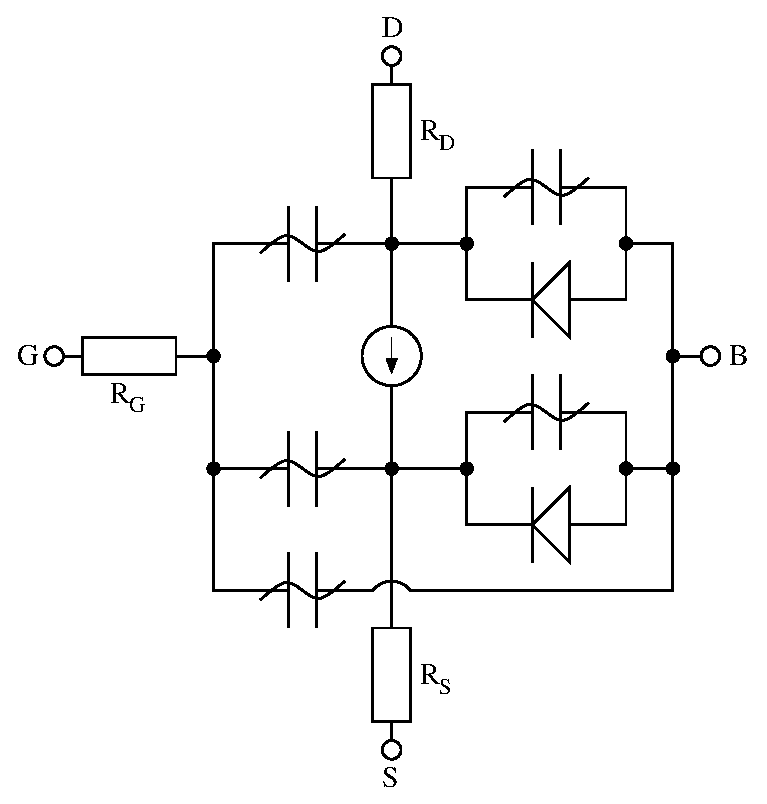
\includegraphics[width=0.6\linewidth]{mosfet}
\end{center}
\caption{n-channel MOSFET large signal model}
\label{fig:mosfet}
\end{figure}
\FloatBarrier

Beforehand some useful abbreviation are made to simplify the DC
current equations.
\begin{align}
L_{eff} &= L - 2\cdot L_D\\
\beta &= K_P\cdot \dfrac{W}{L_{eff}}
\end{align}

The bias-dependent threshold voltage depends on the bulk-source
voltage $V_{BS}$ or the bulk-drain voltage $V_{BD}$ depending on the
mode of operation.
\begin{equation}
V_{Th} = V_{T0} +
\begin{cases}
\begin{array}{ll}
\gamma\cdot\left(\sqrt{\Phi - V_{BS}} - \sqrt{\Phi}\right) & \textrm{ for } V_{DS} \ge 0, \textrm{ i.e. } V_{BS} \ge V_{BD}\\
\gamma\cdot\left(\sqrt{\Phi - V_{BD}} - \sqrt{\Phi}\right) & \textrm{ for } V_{DS} < 0, \textrm{ i.e. } V_{BD} > V_{BS}
\end{array}
\end{cases}
\end{equation}

The following equations describe the DC current behaviour of a
N-channel MOSFET in normal mode, i.e. $V_{DS} > 0$, according to
Shichman and Hodges.

\begin{itemize}
\item cutoff region: $V_{GS} - V_{Th} < 0$
\begin{align}
I_{d} &= 0\\
g_{ds} &= 0\\
g_{m} &= 0\\
g_{mb} &= 0\\
%\end{align}
\intertext{
\item saturation region: $0 < V_{GS} - V_{Th} < V_{DS}$
}
%\begin{align}
I_{d} &= \beta / 2 \cdot \left(1 + \lambda V_{DS}\right) \cdot\left(V_{GS} - V_{Th}\right)^{2}\\
g_{ds} &= \beta / 2 \cdot \lambda\left(V_{GS} - V_{Th}\right)^{2}\\
g_{m} &= \beta \cdot\left(1 + \lambda V_{DS}\right) \left(V_{GS} - V_{Th}\right)\\
g_{mb} &= g_m\cdot\dfrac{\gamma}{2\sqrt{\Phi - V_{BS}}}\\
%\end{align}
\intertext{
\item linear region: $V_{DS} < V_{GS} - V_{Th}$
}
%\begin{align}
I_{d} &= \beta\cdot\left(1 + \lambda V_{DS}\right)\cdot\left(V_{GS} - V_{Th} - V_{DS}/2\right)\cdot V_{DS}\\
g_{ds} &= \beta\cdot\left(1 + \lambda V_{DS}\right)\cdot \left(V_{GS} - V_{Th} - V_{DS}\right) + \beta \cdot \lambda V_{DS}\cdot\left(V_{GS} - V_{Th} - V_{DS} / 2\right)\\
g_{m} &= \beta\cdot\left(1 + \lambda V_{DS}\right)\cdot V_{DS}\\
g_{mb} &= g_m\cdot\dfrac{\gamma}{2\sqrt{\Phi - V_{BS}}}
\end{align}
\end{itemize}

with
\begin{equation}
g_{ds} = \dfrac{\partial I_d}{\partial V_{DS}}
\;\;\;\; \textrm{ and } \;\;\;\;
g_{m} = \dfrac{\partial I_d}{\partial V_{GS}}
\;\;\;\; \textrm{ and } \;\;\;\;
g_{mb} = \dfrac{\partial I_d}{\partial V_{BS}}
\end{equation}

In the inverse mode of operation, i.e. $V_{DS} < 0$, the same
equations can be applied with the following modifications.  Replace
$V_{BS}$ with $V_{BD}$, $V_{GS}$ with $V_{GD}$ and $V_{DS}$ with
$-V_{DS}$.  The drain current $I_d$ gets reversed.  Furthermore the
transconductances alter their controlling nodes, i.e.
\begin{equation}
g_{m} = \dfrac{\partial I_d}{\partial V_{GD}}
\;\;\;\; \textrm{ and } \;\;\;\;
g_{mb} = \dfrac{\partial I_d}{\partial V_{BD}}
\end{equation}

The current equations of the two parasitic diodes at the bulk node and
their derivatives write as follows.
\begin{align}
I_{BD} &= I_{SD}\cdot \left(e^{\frac{V_{BD}}{N\cdot V_T}} - 1\right) &
g_{bd} &= \dfrac{\partial I_{BD}}{\partial V_{BD}} = \dfrac{I_{SD}}{N\cdot V_T}\cdot e^{\frac{V_{BD}}{N\cdot V_T}}\\
I_{BS} &= I_{SS}\cdot \left(e^{\frac{V_{BS}}{N\cdot V_T}} - 1\right) &
g_{bs} &= \dfrac{\partial I_{BS}}{\partial V_{BS}} = \dfrac{I_{SS}}{N\cdot V_T}\cdot e^{\frac{V_{BS}}{N\cdot V_T}}
\end{align}

with
\begin{equation}
I_{SD} = I_S
\;\;\;\; \textrm{ and } \;\;\;\;
I_{SS} = I_S
\end{equation}

\begin{figure}[ht]
\begin{center}
\includegraphics[width=0.7\linewidth]{dcmosfet}
\end{center}
\caption{accompanied DC model of intrinsic MOSFET}
\label{fig:dcmosfet}
\end{figure}
\FloatBarrier

With the accompanied DC model shown in fig. \ref{fig:dcmosfet} it is
possible to form the MNA matrix and the current vector of the
intrinsic MOSFET device.
\begin{equation}
\begin{bmatrix}
0 & 0 & 0 & 0\\
g_{m} & g_{ds} + g_{bd} & -g_{ds} - g_{m} -g_{mb} & g_{mb} - g_{bd}\\
-g_{m} & -g_{ds} & g_{bs} + g_{ds} + g_{m} + g_{mb} & -g_{bs} - g_{mb}\\
0 & -g_{bd} & -g_{bs} & g_{bs} + g_{bd}\\
\end{bmatrix}
\cdot
\begin{bmatrix}
V_{G}\\
V_{D}\\
V_{S}\\
V_{B}\\
\end{bmatrix}
=
\begin{bmatrix}
0\\
+I_{BD_{eq}} - I_{DS_{eq}}\\
+I_{BS_{eq}} + I_{DS_{eq}}\\
-I_{BD_{eq}} - I_{BS_{eq}}\\
\end{bmatrix}
\end{equation}

\begin{align}
I_{BD_{eq}} &= I_{BD} - g_{bd} \cdot V_{BD}\\
I_{BS_{eq}} &= I_{BS} - g_{bs} \cdot V_{BS}\\
I_{DS_{eq}} &= I_{d} - g_{m} \cdot V_{GS} - g_{mb} \cdot V_{BS} - g_{ds}\cdot V_{DS}
\end{align}

\subsection{Physical model}
%\addcontentsline{toc}{subsection}{Physical model}

There are electrical parameters as well as physical and geometry
parameters in the set of model parameters for the MOSFETs ``First
Order Model''.  Some of the electrical parameters can be derived from
the geometry and physical parameters.

\addvspace{12pt}

The oxide capacitance per square meter of the channel area can be
computed as
\begin{equation}
C'_{ox} = \varepsilon_0\cdot\dfrac{\varepsilon_{ox}}{T_{ox}}
\;\;\;\; \textrm{ with } \;\;\;\;
\varepsilon_{ox} = \varepsilon_{SiO_2} = 3.9
\end{equation}

Then the overall oxide capacitance can be written as
\begin{equation}
C_{ox} = C'_{ox}\cdot W \cdot L_{eff}
\end{equation}

The transconductance coefficient $K_P$ can be calculated using
\begin{equation}
K_P = \mu_0\cdot C'_{ox}
\end{equation}

The surface potential $\Phi$ is given by (with temperature voltage $V_T$)
\begin{equation}
\Phi = 2\cdot V_T\cdot \ln{\left(\dfrac{N_{SUB}}{n_i}\right)}
\;\;\;\; \textrm{ with the intrinsic density } \;
n_i = 1.45\cdot 10^{16} 1/\meter^3
\label{eq:PhiMOS}
\end{equation}

Equation \eqref{eq:PhiMOS} holds for acceptor concentrations $N_A$
($N_{SUB}$) essentially greater than the donor concentration $N_D$.
The bulk threshold $\gamma$ (also sometimes called the body effect
coefficient) is
\begin{equation}
\gamma = \dfrac{\sqrt{2\cdot e\cdot \varepsilon_{Si}\cdot \varepsilon_{0}\cdot N_{SUB}}}{C'_{ox}}
\;\;\;\; \textrm{ with } \;\;\;\;
\varepsilon_{Si} = 11.7
\end{equation}

And finally the zero-bias threshold voltage $V_{T0}$ writes as
follows.
\begin{equation}
V_{T0} = V_{FB} + \Phi + \gamma\cdot\sqrt{\Phi}
\end{equation}

Whereas $V_{FB}$ denotes the flat band voltage consisting of the work
function difference $\Phi_{MS}$ between the gate and substrate
material and an additional potential due to the oxide surface charge.
\begin{equation}
V_{FB} = \Phi_{MS} - \dfrac{e\cdot N_{SS}}{C'_{ox}}
\end{equation}

The temperature dependent bandgap potential $E_{G}$ of silicon
(substrate material Si) writes as follows.  With $T = 290\kelvin$ the
bandgap is approximately $1.12eV$.
\begin{equation}
E_{G}\left(T\right) = 1.16 - \dfrac{7.02\cdot 10^{-4}\cdot T^2}{T + 1108}
\end{equation}

The work function difference $\Phi_{MS}$ gets computed dependent on
the gate conductor material.  This can be either alumina ($\Phi_{M} =
4.1eV$), n-polysilicon ($\Phi_{M} \approx 4.15eV$) or p-polysilicon
($\Phi_{M} \approx 5.27eV$).  The work function of a semiconductor,
which is the energy difference between the vacuum level and the Fermi
level (see fig. \ref{fig:mosband}), varies with the doping
concentration.
\begin{equation}
\Phi_{MS} = \Phi_{M} - \Phi_{S} = \Phi_{M} - \left(4.15 + \dfrac{1}{2}E_{G} + \dfrac{1}{2}\Phi\right)
\label{eq:workfunction}
\end{equation}
\begin{equation}
\Phi_{M} =
\begin{cases}
\begin{array}{ll}
4.1 & \textrm{ for } T_{PG} = +0, \textrm{ i.e. alumina}\\
4.15 & \textrm{ for } T_{PG} = +1, \textrm{ i.e. opposite to bulk }\\
4.15 + E_{G} & \textrm{ for } T_{PG} = -1, \textrm{ i.e. same as bulk }\\
\end{array}
\end{cases}
\end{equation}

\begin{figure}[ht]
\begin{center}
\psfrag{XAl}{$\mathsmaller{\mathrm{\chi_{Al}}}$}
\psfrag{XSi}{$\mathsmaller{\mathrm{\chi_{Si}}}$}
\psfrag{E0}{$\mathsmaller{\mathrm{E_0}}$}
\psfrag{Ec}{$\mathsmaller{\mathrm{E_C}}$}
\psfrag{Ev}{$\mathsmaller{\mathrm{E_V}}$}
\psfrag{Ef}{$\mathsmaller{\mathrm{E_F}}$}
\psfrag{Ei}{$\mathsmaller{\mathrm{E_I}}$}
\psfrag{Eg}{$\mathsmaller{\mathrm{E_G}}$}
\psfrag{Phi}{$\mathsmaller{\mathrm{\frac{1}{2}\Phi}}$}
\includegraphics[width=0.95\linewidth]{mosband}
\end{center}
\caption{energy band diagrams of isolated (flat band) MOS materials}
\label{fig:mosband}
\end{figure}
\FloatBarrier

The expression in eq. \eqref{eq:workfunction} is visualized in
fig. \ref{fig:mosband}.  The abbreviations denote

\addvspace{12pt}

\begin{tabular}{rl}
$\chi_{Al}$ & electron affinity of alumina $= 4.1eV$\\
$\chi_{Si}$ & electron affinity of silicon $= 4.15eV$\\
$E_0$ & vacuum level\\
$E_C$ & conduction band\\
$E_V$ & valence band\\
$E_F$ & Fermi level\\
$E_I$ & intrinsic Fermi level\\
$E_G$ & bandgap of silicon $\approx 1.12eV$ at room temperature\\
\end{tabular}

\addvspace{12pt}

Please note that the potential $1/2\cdot \Phi$ is positive in p-MOS
and negative in n-MOS as the following equation reveals.
\begin{equation}
\Phi_F = \dfrac{E_F - E_I}{e}
\end{equation}

When the gate conductor material is a heavily doped polycrystalline
silicon (also called polysilicon) then the model assumes that the
Fermi level of this semiconductor is the same as the conduction band
(for n-poly) or the valence band (for p-poly).  In alumina the Fermi
level, valence and conduction band all equal the electron affinity.

\addvspace{12pt}

If the zero-bias bulk junction bottom capacitance per square meter of
junction area $C_J$ is not given it can be computed as follows.
\begin{equation}
C_J = \sqrt{\dfrac{\varepsilon_{Si}\cdot \varepsilon_{0}\cdot e\cdot N_{SUB}}{2\cdot \Phi_B}}
\end{equation}

That's it for the physical parameters.  The geometry parameters
account for the electrical parameters per length, area or volume.
Thus the MOS model is scalable.

\addvspace{12pt}

The diffusion resistances at drain and gate are computed as follows.
The sheet resistance $R_{SH}$ refers to the thickness of the diffusion
area.
\begin{equation}
R_D = N_{RD}\cdot R_{SH}
\;\;\;\; \textrm{ and } \;\;\;\;
R_S = N_{RS}\cdot R_{SH}
\end{equation}

If the bulk junction saturation current per square meter of the
junction area $J_S$ and the drain and source areas are given the
according saturation currents are calculated with the following
equations.
\begin{equation}
I_{SD} = A_{D}\cdot J_{S}
\;\;\;\; \textrm{ and } \;\;\;\;
I_{SS} = A_{S}\cdot J_{S}
\end{equation}

If the parameters $C_{BD}$ and $C_{BS}$ are not given the zero-bias
depletion capacitances for the bottom and sidewall capacitances are
computed as follows.
\begin{align}
C_{BD} &= C_{J}\cdot A_D\\
C_{BS} &= C_{J}\cdot A_S\\
C_{BDS} &= C_{JSW}\cdot P_D\\
C_{BSS} &= C_{JSW}\cdot P_S
\end{align}

\subsection{Small signal model}
%\addcontentsline{toc}{subsection}{Small signal model}
\label{sec:SmallSignalMOS}

\begin{figure}[ht]
\begin{center}
\includegraphics[width=0.7\linewidth]{spmosfet}
\end{center}
\caption{small signal model of intrinsic MOSFET}
\label{fig:spmosfet}
\end{figure}
\FloatBarrier

The bulk-drain and bulk-source capacitances in the MOSFET model split
into three parts: the junctions depletion capacitance which consists
of an area and a sidewall part and the diffusion capacitance.

\begin{align}
C_{BD_{dep}} &= 
\begin{cases}
\begin{array}{ll}
C_{BD}\cdot \left(1 - \dfrac{V_{BD}}{\Phi_{B}}\right)^{-M_{J}} & \textrm{ for } V_{BD} \le F_{C}\cdot \Phi_{B}\\
\dfrac{C_{BD}}{\left(1 - F_{C}\right)^{M_{J}}}\cdot \left(1 + \dfrac{M_{J}\cdot \left(V_{BD} - F_{C}\cdot \Phi_{B}\right)}{\Phi_{B}\cdot \left(1 - F_{C}\right)}\right) & \textrm{ for } V_{BD} > F_{C}\cdot \Phi_{B}
\end{array}
\end{cases}\\
C_{BDS_{dep}} &= 
\begin{cases}
\begin{array}{ll}
C_{BDS}\cdot \left(1 - \dfrac{V_{BD}}{\Phi_{B}}\right)^{-M_{JSW}} & \textrm{ for } V_{BD} \le F_{C}\cdot \Phi_{B}\\
\dfrac{C_{BDS}}{\left(1 - F_{C}\right)^{M_{JSW}}}\cdot \left(1 + \dfrac{M_{JSW}\cdot \left(V_{BD} - F_{C}\cdot \Phi_{B}\right)}{\Phi_{B}\cdot \left(1 - F_{C}\right)}\right) & \textrm{ for } V_{BD} > F_{C}\cdot \Phi_{B}
\end{array}
\end{cases}\\
C_{BS_{dep}} &= 
\begin{cases}
\begin{array}{ll}
C_{BS}\cdot \left(1 - \dfrac{V_{BS}}{\Phi_{B}}\right)^{-M_{J}} & \textrm{ for } V_{BS} \le F_{C}\cdot \Phi_{B}\\
\dfrac{C_{BS}}{\left(1 - F_{C}\right)^{M_{J}}}\cdot \left(1 + \dfrac{M_{J}\cdot \left(V_{BS} - F_{C}\cdot \Phi_{B}\right)}{\Phi_{B}\cdot \left(1 - F_{C}\right)}\right) & \textrm{ for } V_{BS} > F_{C}\cdot \Phi_{B}
\end{array}
\end{cases}\\
C_{BSS_{dep}} &= 
\begin{cases}
\begin{array}{ll}
C_{BSS}\cdot \left(1 - \dfrac{V_{BS}}{\Phi_{B}}\right)^{-M_{JSW}} & \textrm{ for } V_{BS} \le F_{C}\cdot \Phi_{B}\\
\dfrac{C_{BSS}}{\left(1 - F_{C}\right)^{M_{JSW}}}\cdot \left(1 + \dfrac{M_{JSW}\cdot \left(V_{BS} - F_{C}\cdot \Phi_{B}\right)}{\Phi_{B}\cdot \left(1 - F_{C}\right)}\right) & \textrm{ for } V_{BS} > F_{C}\cdot \Phi_{B}
\end{array}
\end{cases}
\end{align}

The diffusion capacitances of the bulk-drain and bulk-source junctions
are determined by the transit time of the minority charges through the
junction.
\begin{align}
C_{BD_{diff}} &= g_{bd}\cdot T_T\\
C_{BS_{diff}} &= g_{bs}\cdot T_T
\end{align}

Charge storage in the MOSFET consists of capacitances associated with
parasitics and the intrinsic device.  Parasitic capacitances consist
of three constant overlap capacitances.  The intrinsic capacitances
consist of the nonlinear thin-oxide capacitance, which is distributed
among the gate, drain, source and bulk regions.  The MOS gate
capacitances, as a nonlinear function of the terminal voltages, are
modeled by J.E. Meyer's piece-wise linear model \cite{Meyer}.

\addvspace{12pt}

The bias-dependent gate-oxide capacitances distribute according to the
Meyer model \cite{Meyer} as follows.

\begin{itemize}
\item cutoff regions: $V_{GS} - V_{Th} < 0$
\begin{itemize}
\item $V_{GS} - V_{Th} \le -\Phi$
\begin{align}
C_{GS} &= 0\\
C_{GD} &= 0\\
C_{GB} &= C_{ox}\\
%\end{align}
\intertext{
\item $-\Phi < V_{GS} - V_{Th} \le -\Phi / 2$
}
%\begin{align}
C_{GS} &= 0\\
C_{GD} &= 0\\
C_{GB} &= -C_{ox}\cdot\dfrac{V_{GS} - V_{Th}}{\Phi}\\
%\end{align}
\intertext{
\item $-\Phi / 2 < V_{GS} - V_{Th} \le 0$
}
%\begin{align}
C_{GS} &= \dfrac{2}{3}\cdot C_{ox} + \dfrac{4}{3}\cdot C_{ox}\cdot\dfrac{V_{GS} - V_{Th}}{\Phi}\\
C_{GD} &= 0\\
C_{GB} &= -C_{ox}\cdot\dfrac{V_{GS} - V_{Th}}{\Phi}
\end{align}
\end{itemize}
\item saturation region: $0 < V_{GS} - V_{Th} < V_{DS}$
\begin{align}
C_{GS} &= \dfrac{2}{3}\cdot C_{ox}\\
C_{GD} &= 0\\
C_{GB} &= 0\\
%\end{align}
\intertext{
\item linear region: $V_{DS} < V_{GS} - V_{Th}$
}
%\begin{align}
C_{GS} &= \dfrac{2}{3}\cdot C_{ox}\cdot \left(1 - \dfrac{\left(V_{Dsat} - V_{DS}\right)^2}{\left(2\cdot V_{Dsat} - V_{DS}\right)^2}\right)\\
C_{GD} &= \dfrac{2}{3}\cdot C_{ox}\cdot \left(1 - \dfrac{V_{Dsat}^2}{\left(2\cdot V_{Dsat} - V_{DS}\right)^2}\right)\\
C_{GB} &= 0
%\end{align}
\end{align}
\end{itemize}

with
\begin{equation}
V_{Dsat} =
\begin{cases}
\begin{array}{ll}
V_{GS} - V_{Th} & \textrm{ for } V_{GS} - V_{Th} > 0\\
0 & \textrm{ otherwise }
\end{array}
\end{cases}
\end{equation}

In the inverse mode of operation $V_{GS}$ and $V_{GD}$ need to be
exchanged, $V_{DS}$ changes its sign, then the above formulas can be
applied as well.

\addvspace{12pt}

The constance overlap capacitances compute as follows.
\begin{align}
C_{GS_{OVL}} &= C_{GSO}\cdot W\\
C_{GD_{OVL}} &= C_{GDO}\cdot W\\
C_{GB_{OVL}} &= C_{GBO}\cdot L_{eff}
\end{align}

With these definitions it is possible to form the small signal
Y-parameter matrix of the intrinsic MOSFET device in an operating
point which can be converted into S-parameters.
\begin{equation}
Y =
\begin{bmatrix}
\parbox[t]{2.0cm}{\centering $Y_{GS} + Y_{GD} + Y_{GB}$} & -Y_{GD} & -Y_{GS} & -Y_{GB}\\
g_{m} - Y_{GD} & Y_{GD} + Y_{BD} + Y_{DS} & -Y_{DS} - g_{m} - g_{mb} & -Y_{BD} + g_{mb}\\
-g_{m} - Y_{GS} & -Y_{DS} & \parbox[t]{2.5cm}{\centering $Y_{GS} + Y_{DS} + Y_{BS} + g_{m} + g_{mb}$} & -Y_{BS} - g_{mb}\\
-Y_{GB} & -Y_{BD} & -Y_{BS} & Y_{BD} + Y_{BS} + Y_{GB}\\
\end{bmatrix}
\end{equation}

with
\begin{align}
Y_{GS} &= j\omega \left(C_{GS} + C_{GS_{OVL}}\right)\\
Y_{GD} &= j\omega \left(C_{GD} + C_{GD_{OVL}}\right)\\
Y_{GB} &= j\omega \left(C_{GB} + C_{GB_{OVL}}\right)\\
Y_{BD} &= g_{bd} + j\omega \left(C_{BD_{dep}} + C_{BDS_{dep}} + C_{BD_{diff}}\right)\\
Y_{BS} &= g_{bs} + j\omega \left(C_{BS_{dep}} + C_{BSS_{dep}} + C_{BS_{diff}}\right)\\
Y_{DS} &= g_{ds}
\end{align}

\subsection{Noise model}
%\addcontentsline{toc}{subsection}{Noise model}

The thermal noise generated by the external resistors $R_G$, $R_S$ and
$R_D$ is characterized by the following spectral density.
\begin{equation}
\dfrac{\overline{i_{R_G}^2}}{\Delta f} = \dfrac{4 k_B T}{R_G}
\;\;\;\; \textrm{ and } \;\;\;\;
\dfrac{\overline{i_{R_D}^2}}{\Delta f} = \dfrac{4 k_B T}{R_D}
\;\;\;\; \textrm{ and } \;\;\;\;
\dfrac{\overline{i_{R_S}^2}}{\Delta f} = \dfrac{4 k_B T}{R_S}
\end{equation}

\begin{figure}[ht]
\begin{center}
\includegraphics[width=0.73\linewidth]{noisemosfet}
\end{center}
\caption{noise model of intrinsic MOSFET}
\label{fig:noisemosfet}
\end{figure}
\FloatBarrier

Channel and flicker noise generated by the DC transconductance $g_m$
and current flow from drain to source is characterized by the spectral
density
\begin{equation}
\dfrac{\overline{i_{ds}^2}}{\Delta f} = \dfrac{8 k_B T g_m}{3} + K_F\dfrac{I_{DS}^{A_F}}{f^{F_{FE}}}
\end{equation}

The noise current correlation matrix (admittance representation) of
the intrinsic MOSFET can be expressed as
\begin{equation}
\underline{C}_Y = \Delta f
\begin{bmatrix}
0 & 0 & 0 & 0\\
0 & +\overline{i_{ds}^2} & -\overline{i_{ds}^2} & 0\\
0 & -\overline{i_{ds}^2} & +\overline{i_{ds}^2} & 0\\
0 & 0 & 0 & 0\\
\end{bmatrix}
\end{equation}

This matrix representation can be easily converted to the noise-wave
representation $\underline{C}_S$ if the small signal S-parameter
matrix is known.
